\documentclass[../SWD_disp.tex]{subfiles}

\begin{document}
\section{Observer Pattern}

Giv definitionen af et design pattern til at starte med.

\subsection{Opbygning af Observer Pattern}
Observer Pattern er i gruppen af behavioral patterns, fordi den denfinerer måden for kommunkationen mellem klasserne.
\\

Det tillate et enkelt object kendt som "subject" til, at publiserer ændringer i dens state. En eller mange observer objekter der afhænger af subjects, kan subscribe til et, således at de automatisk bliver notificeret.
\\

Observer Pattern giver lav koblint mellem subjects og observers
\\

Provider (data der ændres) og Consumer (data der skal hentes fra provider)
\begin{itemize}
    \item Vi skal kunne tillate consumeren til at blive tilføjet (attached) til provideren uden, at ændre implementeringsmæssigt for Procider (OCP)
    \item Tillade provideren til at informaerer consumers ved data ændring (lav kobling)
    \item Tillage mange consumers til, at blive informeret på opdatering af den samme data.
    \item Se efter 1-many afhængigheder således, at når det ene object ændrer state, til dens afhængige blive notificeret og opdateret automatisk.
\end{itemize}

\begin{figure}[H]
    \centering
    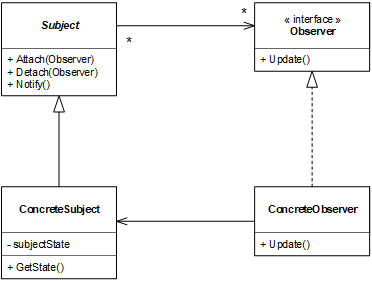
\includegraphics{observer_pattern.PNG}
    \caption{Observer Pattern}
    \label{fig:observer_pattern}
\end{figure}

\begin{table}[H]
    \centering
    \begin{tabular}{l|p{0.7\textwidth}}
        Klasse          & Beskrivelse        \\ \toprule
        ConcreteSubject                & Har dens egen state. Når der sker ændring i state, vil objecktet kalde på base klassens Notify metode for, at indikere det til alle den observere. Dat observernes funktionalitet er ukendt for base klassen (subject), giver concrete subject mulighed for observerne, at læse den opdatetrede state. I dette tilfælde via en \textbf{GetState()}, som er provideren.   \\ \midrule
        Subject         & Dette er en abstrakt base klasse for \textbf{ConcreteSubject}. Består af Attach til at tilføje nye observers, samt Detach til at fjerne eksisterende observers. Indeholder en metode \textbf{Notify()} det kan bliver kaldt ved ændring i ConcreteSubject's state, så observers kan blive notificeret. Denne Notify metoder looper igennem alle de registrerede observers, ved at kalde deres update metode.           \\ \midrule
        Observer(interface)    & Dette er en abstrakt base klasse for alle observers, der definerer en metoder der bliver kaldt, når en state ændres.             \\ \midrule
        ConcreteObserver & De konkrete observers er subscribers, der reagerer når der sker en ændring i subject's state. Når \textbf{Update()} bliver kaldt, vil den undersøge subjektet for at bestemmet hvilke ændringer der er sket. I dette tilfølge er dette vores consumer. \\ \bottomrule
    \end{tabular}
    \caption{sammenligning af WPF og UWP}\label{tab:wpfVSuwp}
\end{table}

Fremmer godt software design ved at anvende SOLID principper. OCP = lav koblint mellem Provider og Consumer. Let at teste.

\subsection*{Fordele}
\begin{itemize}
    \item Skaber lav kobling mellem provider og consumer objekter.
    \item Tillader at opdaterer data på mange objekter samtidigt, på en effektiv måde.
    \item Ingen behov for, at modificerer på et objekt ved tilføjelse af nye observers. Dette er pga. OCP.
    \item Tilføje og fjerne eksisterende observers til enhver tid.
\end{itemize}

\subsection*{Ulemper}
\begin{itemize}
    \item Uden omtankte og brug af dette pattern i et forkert kontekst, kan man tilføje unødvendig kompleksitet.
    \item Rækkefølgen af notifications af observers er uafhængig.
\end{itemize}

\subsection*{Forskellige varianter af GoF Observer}
\subsubsection*{Subject af samme type}
\begin{figure}[H]
    \centering
    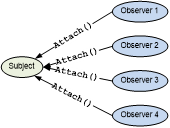
\includegraphics[scale = 1.5]{subject_same_type.PNG}
    \caption{Subject Same Type}
    \label{fig:subject_same_type}
\end{figure}


\subsubsection*{Ved samme type implementering}
\begin{figure}[H]
    \centering
    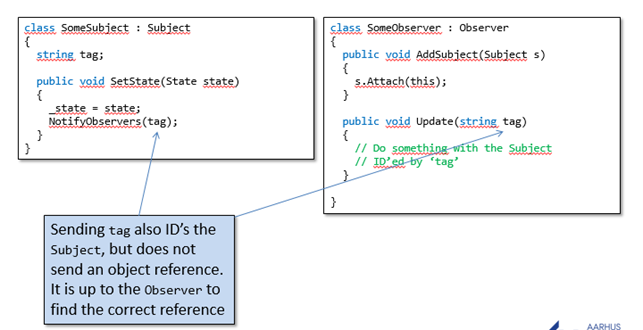
\includegraphics{same_type_impl.PNG}
    \caption{Samme Type Implementering}
    \label{fig:same_type_impl}
\end{figure}

\subsubsection*{Ved håndtering af subjekt af forskellige typer:}
\begin{figure}[H]
    \centering
    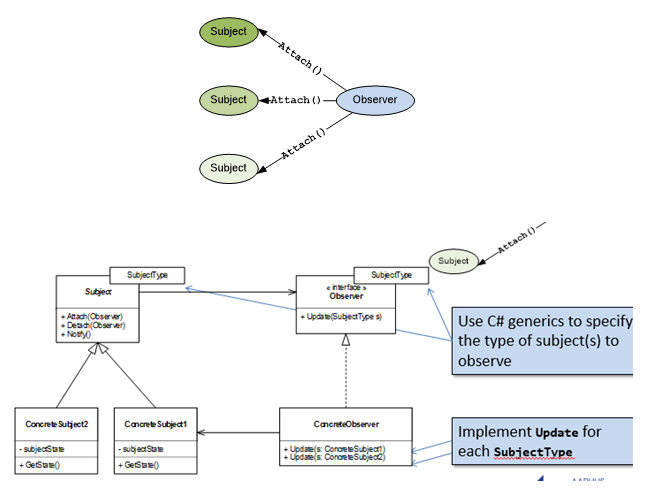
\includegraphics{subject_different_type.PNG}
    \caption{Subject af forskellige typer}
    \label{fig:subject_diff_type}
\end{figure}
\end{document}
